
\documentclass[11pt]{article}

\usepackage[T1]{fontenc}
\usepackage[utf8]{inputenc}
\usepackage{lmodern}
\usepackage[a4paper,top=0.72in,bottom=0.78in,left=0.72in,right=0.72in]{geometry}
\usepackage{microtype}
\usepackage{amsmath,amssymb,mathtools}
\usepackage{booktabs,tabularx,array,multirow}
\usepackage{enumitem}
\usepackage{xcolor}
\usepackage{tikz}
\usetikzlibrary{positioning,arrows.meta,calc,fit,backgrounds,shapes.geometric,decorations.pathmorphing}
\usepackage[most]{tcolorbox}
\usepackage{listings}
\usepackage{caption}
\usepackage{fancyhdr}
\usepackage{hyperref}
\usepackage{lastpage}

\definecolor{ink}{HTML}{0B1020}
\definecolor{navy}{HTML}{111A35}
\definecolor{royal}{HTML}{202B5C}
\definecolor{violet}{HTML}{7567FF}
\definecolor{cyan}{HTML}{13BFEA}
\definecolor{gold}{HTML}{B98A22}
\definecolor{palegold}{HTML}{FFF7DD}
\definecolor{mint}{HTML}{DFF8EF}
\definecolor{rose}{HTML}{FFE7EB}
\definecolor{ice}{HTML}{F5F8FF}
\definecolor{line}{HTML}{D8DEEA}
\definecolor{zkg}{HTML}{EAF2FF}
\definecolor{dark}{HTML}{050713}

\hypersetup{colorlinks=true, linkcolor=royal, citecolor=royal, urlcolor=royal, pdftitle={GoalOS V97.4: Private On-Chain Validated Skill Graphs}, pdfauthor={Montreal.AI Research}}
\pagestyle{fancy}
\fancyhf{}
\lhead{\small\scshape GoalOS V97.4}
\chead{\small Private On-Chain Validated Skill Graphs}
\rhead{\small\scshape Research Draft}
\cfoot{\small\thepage\,/\,\pageref{LastPage}}
\renewcommand{\headrulewidth}{0.35pt}
\renewcommand{\footrulewidth}{0pt}
\setlength{\headheight}{14pt}
\setlength{\parskip}{5.5pt}
\setlength{\parindent}{0pt}

\captionsetup{font=small,labelfont={bf,color=royal},labelsep=period}
\setlist[itemize]{leftmargin=1.35em,itemsep=2pt,topsep=3pt,label=\textcolor{violet}{\scriptsize$\blacklozenge$}}
\setlist[enumerate]{leftmargin=1.5em,itemsep=2pt,topsep=3pt}
\renewcommand{\arraystretch}{1.22}
\newcolumntype{Y}{>{\raggedright\arraybackslash}X}
\newcommand{\term}[1]{\textsc{#1}}
\newcommand{\code}[1]{\texttt{#1}}

\tcbset{
  sharp corners=downhill,
  enhanced,
  boxrule=0.45pt,
  colback=ice,
  colframe=line,
  arc=3mm,
  left=8pt,right=8pt,top=7pt,bottom=7pt
}
\newtcolorbox{thesisbox}[1]{colback=palegold,colframe=gold,title={#1},fonttitle=\bfseries\scshape,coltitle=ink}
\newtcolorbox{defbox}[1]{colback=zkg,colframe=cyan,title={#1},fonttitle=\bfseries\scshape,coltitle=ink}
\newtcolorbox{warnbox}[1]{colback=rose,colframe=red,title={#1},fonttitle=\bfseries\scshape,coltitle=ink}
\newtcolorbox{lawbox}[1]{colback=mint,colframe=green!50!black,title={#1},fonttitle=\bfseries\scshape,coltitle=ink}

\lstdefinestyle{json}{
  basicstyle=\ttfamily\footnotesize,
  breaklines=true,
  breakatwhitespace=true,
  columns=fullflexible,
  showstringspaces=false,
  frame=single,
  rulecolor=\color{line},
  backgroundcolor=\color{ice},
  xleftmargin=2pt,
  xrightmargin=2pt,
  aboveskip=5pt,
  belowskip=5pt
}
\lstset{style=json}

% TikZ styles
\tikzset{
  nodebox/.style={draw=line, rounded corners=4pt, align=center, fill=white, minimum height=0.72cm, inner xsep=6pt, inner ysep=4pt, font=\scriptsize},
  strongbox/.style={draw=royal, rounded corners=4pt, align=center, fill=ice, minimum height=0.72cm, inner xsep=6pt, inner ysep=4pt, font=\scriptsize\bfseries},
  goodbox/.style={draw=green!45!black, rounded corners=4pt, align=center, fill=mint, minimum height=0.72cm, inner xsep=6pt, inner ysep=4pt, font=\scriptsize},
  warnnode/.style={draw=gold, rounded corners=4pt, align=center, fill=palegold, minimum height=0.72cm, inner xsep=6pt, inner ysep=4pt, font=\scriptsize},
  badbox/.style={draw=red!60!black, rounded corners=4pt, align=center, fill=rose, minimum height=0.72cm, inner xsep=6pt, inner ysep=4pt, font=\scriptsize},
  chainarrow/.style={-{Stealth[length=2.2mm,width=1.6mm]}, thick, draw=violet},
  proofarrow/.style={-{Stealth[length=2.2mm,width=1.6mm]}, thick, draw=cyan!70!black},
  gatearrow/.style={-{Stealth[length=2.2mm,width=1.6mm]}, thick, draw=gold!80!black},
  repairarrow/.style={-{Stealth[length=2.0mm,width=1.4mm]}, dashed, thick, draw=red!70!black},
  softarrow/.style={-{Stealth[length=2.0mm,width=1.4mm]}, dashed, draw=gold!80!black}
}

\begin{document}

\begin{titlepage}
\thispagestyle{empty}
\begin{tikzpicture}[remember picture,overlay]
  \fill[white] (current page.south west) rectangle (current page.north east);
  \shade[inner color=cyan!10,outer color=white] ($(current page.center)+(0,2.2)$) circle (7.4cm);
  \draw[gold!35, line width=0.5pt] ($(current page.center)+(0,2.2)$) circle (4.25cm);
  \draw[cyan!30, line width=0.4pt, dashed] ($(current page.center)+(0,2.2)$) circle (5.3cm);
  \draw[violet!25, line width=0.4pt] ($(current page.center)+(0,2.2)$) circle (6.1cm);
  \foreach \a/\r/\c in {15/4.25/gold,70/5.3/cyan,135/6.1/violet,205/5.3/cyan,290/4.25/gold}{
    \fill[\c!75] ($(current page.center)+(0,2.2)+(\a:\r)$) circle (1.35pt);
  }
\end{tikzpicture}
\vspace*{1.0cm}
\begin{center}
  {\Large\scshape Montreal.AI Research}\par
  \vspace{1.15cm}
  {\fontsize{34}{38}\selectfont\bfseries\color{ink} GoalOS V97.4}\par
  \vspace{0.18cm}
  {\fontsize{24}{30}\selectfont\bfseries\color{royal} Private On-Chain}\par
  {\fontsize{24}{30}\selectfont\bfseries\color{royal} Validated Skill Graph}\par
  \vspace{0.55cm}
  {\Large\itshape\color{ink} ENS-Gated Agent Writes, Encrypted Skill Capsules, and Zero-Knowledge Chronicle Authority}\par
  \vspace{0.8cm}
  \rule{0.42\linewidth}{0.45pt}\par
  \vspace{0.9cm}
\end{center}

\begin{thesisbox}{Design law}
GoalOS V97.4 secures the Validated Skill Graph as Ethereum mainnet proof commitments and optional encrypted on-chain capsules. Direct AGI Agents - wallets that own \code{*.agent.agi.eth} - may write, supersede, or revoke skill commitments. Private intelligence is never written as plaintext. If it must live on-chain, it is written as ciphertext plus commitments; zero-knowledge proofs attest policy satisfaction without revealing the capsule.
\end{thesisbox}

\vfill
\begin{center}
\begin{minipage}{0.86\linewidth}
\small\color{ink}
\textbf{Claim boundary.} This paper defines a research and implementation architecture. It does not claim achieved AGI, achieved ASI, empirical state of the art, legal certification, financial advice, live settlement, or production authority. Ethereum mainnet deployment, cryptography, smart contracts, zk circuits, key management, and validator operations require independent review.
\end{minipage}
\end{center}
\end{titlepage}

\section*{Abstract}
Frontier models make candidate output abundant. Institutions need something different: proof-carrying memory that can survive replay, validation, scope checks, rollback, and adversarial review. This paper specifies \textbf{GoalOS V97.4}, a mainnet-secured architecture for the \term{Validated Skill Graph}. The architecture stores public proof commitments, evidence roots, ProofBundle roots, schema hashes, version events, and authorization records on Ethereum mainnet. It restricts graph updates to wallets that own direct \code{*.agent.agi.eth} subnames, such as \code{john.agent.agi.eth}, using ENS Registry and NameWrapper ownership checks. It adds a privacy-preserving storage model in which private skill intelligence can be kept as encrypted ciphertext on-chain or off-chain, while zero-knowledge proofs attest hidden policy predicates such as proof-level satisfaction, validator quorum, replay availability, blocked-claim exclusion, and Chronicle eligibility. The result is a proof-governed memory substrate: agents may write only under verifiable identity authority, validators may attest without exposing private skill contents, and future missions may rely only on Chronicle-admitted capability.

\begin{thesisbox}{Executive summary}
The durable unit is not a prompt or transcript. It is a validated skill: a scoped, replayable, evidence-backed capability admitted through a policy gate and safe to reuse. V97.4 adds an Ethereum mainnet security layer: direct AGI Agent authorization, encrypted private capsule handling, zero-knowledge policy proofs, and append-auditable commitment events.
\end{thesisbox}

\section{Design Objective}
GoalOS converts autonomous AI output into proof-bearing machine labor. The core loop is:
\[
\begin{aligned}
&\text{Objective}\rightarrow\text{Mission Contract}\rightarrow\text{Proof Debt}\rightarrow\text{AGI Jobs}\rightarrow\text{ProofBundles}\\[-1mm]
&\rightarrow\text{Evidence Docket}\rightarrow\text{Chronicle}\rightarrow\text{Validated Skill}.
\end{aligned}
\]
The Validated Skill Graph is the memory layer of this loop. It should not admit raw language-model output. It should admit capability manifests only when evidence, replay, validation, risk, scope, and rollback conditions pass.

V97.4 addresses a deployment question: how can this graph be secured on Ethereum mainnet without leaking private operational intelligence? The answer is a layered design:
\begin{enumerate}
  \item direct ENS-based write authorization for AGI Agents;
  \item on-chain commitments and optional on-chain encrypted capsules;
  \item zero-knowledge proofs for hidden policy predicates;
  \item EIP-712 typed attestations for validators and agents;
  \item Chronicle gates that convert proof into bounded future mission authority.
\end{enumerate}

\begin{figure}[t]
\centering
\resizebox{0.96\linewidth}{!}{%
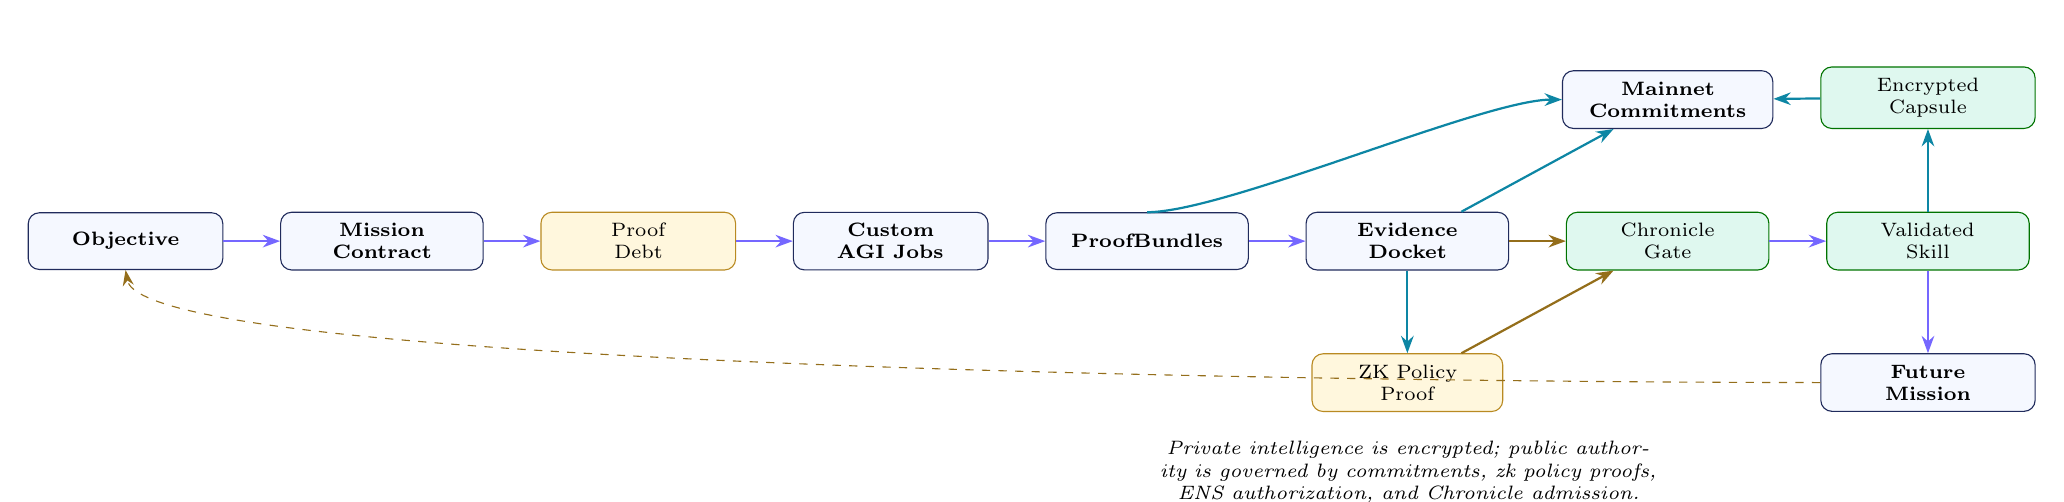
\begin{tikzpicture}[node distance=0.72cm and 0.72cm]
  \node[strongbox, text width=2.05cm] (obj) {Objective};
  \node[strongbox, right=of obj, text width=2.15cm] (mission) {Mission\\Contract};
  \node[warnnode, right=of mission, text width=2.05cm] (debt) {Proof\\Debt};
  \node[strongbox, right=of debt, text width=2.05cm] (jobs) {Custom\\AGI Jobs};
  \node[strongbox, right=of jobs, text width=2.15cm] (bundle) {ProofBundles};
  \node[strongbox, right=of bundle, text width=2.15cm] (docket) {Evidence\\Docket};
  \node[warnnode, below=1.05cm of docket, text width=2.0cm] (zk) {ZK Policy\\Proof};
  \node[goodbox, right=0.72cm of docket, text width=2.15cm] (chron) {Chronicle\\Gate};
  \node[goodbox, right=0.72cm of chron, text width=2.15cm] (skill) {Validated\\Skill};
  \node[strongbox, above=1.05cm of chron, text width=2.25cm] (chain) {Mainnet\\Commitments};
  \node[goodbox, above=1.05cm of skill, text width=2.3cm] (cipher) {Encrypted\\Capsule};
  \node[strongbox, below=1.05cm of skill, text width=2.3cm] (future) {Future\\Mission};
  \draw[chainarrow] (obj) -- (mission);
  \draw[chainarrow] (mission) -- (debt);
  \draw[chainarrow] (debt) -- (jobs);
  \draw[chainarrow] (jobs) -- (bundle);
  \draw[chainarrow] (bundle) -- (docket);
  \draw[gatearrow] (docket) -- (chron);
  \draw[chainarrow] (chron) -- (skill);
  \draw[chainarrow] (skill) -- (future);
  \draw[softarrow] (future.west) .. controls +(180:2.0cm) and +(-80:1.4cm) .. (obj.south);
  \draw[proofarrow] (docket) -- (chain);
  \draw[proofarrow] (bundle.north) .. controls +(0:1.0cm) and +(180:1.0cm) .. (chain.west);
  \draw[proofarrow] (skill) -- (cipher);
  \draw[proofarrow] (cipher) -- (chain);
  \draw[gatearrow] (zk) -- (chron);
  \draw[proofarrow] (docket) -- (zk);
  \node[font=\scriptsize\itshape, text width=8.5cm, align=center, below=0.25cm of zk] {Private intelligence is encrypted; public authority is governed by commitments, zk policy proofs, ENS authorization, and Chronicle admission.};
\end{tikzpicture}}
\caption{GoalOS V97.4 mainnet privacy architecture. Ethereum stores commitments, optional ciphertext capsules, authorization events, and zk proof verification results; Chronicle memory remains proof-gated.}
\label{fig:architecture}
\end{figure}

\section{From Private Intelligence to Verifiable Mainnet Memory}
The phrase ``store intelligence on-chain'' is dangerous if it means plaintext. Ethereum is public, durable, replicated, and adversarially readable. GoalOS therefore distinguishes four storage modes.

\begin{table}[h]
\centering
\small
\begin{tabularx}{\linewidth}{p{0.23\linewidth}Yp{0.28\linewidth}}
\toprule
\textbf{Mode} & \textbf{On-chain material} & \textbf{Use case} \\
\midrule
Commitment-only & Graph root, Evidence Docket root, ProofBundle root, schema hash, version, agent node. & Default mode for sensitive or high-volume intelligence. \\
Encrypted URI & Commitment roots plus pointer to encrypted content-addressed payload. & Practical private graph storage with cheap on-chain verification. \\
Encrypted on-chain capsule & Compact ciphertext stored in contract storage, calldata, or data-availability layer, plus commitments. & High-value compact records requiring public availability of ciphertext. \\
ZK-verified hidden capsule & Public inputs and proof verify policy predicates over a hidden witness. & Prove eligibility without revealing method, evidence, or reviewer notes. \\
\bottomrule
\end{tabularx}
\caption{Storage modes. V97.4 permits encrypted private intelligence on-chain, but never as plaintext; the recommended default is commitment-only or encrypted URI with zk policy proofs.}
\label{tab:storage}
\end{table}

\begin{warnbox}{Privacy correction}
A public blockchain cannot keep plaintext private. GoalOS can keep private intelligence \emph{securely on-chain} only as ciphertext, commitments, and proofs. Long-term confidentiality then depends on encryption choices, key management, access control, revocation policy, and cryptographic assumptions. Highly sensitive raw content should remain encrypted off-chain with on-chain roots and zk proofs.
\end{warnbox}

\section{Direct AGI Agent Authorization}
Write access is restricted to wallets that own a direct subname under \code{agent.agi.eth}. For a label \(\lambda\), such as \code{john}, define:
\[
\mathrm{labelhash}(\lambda) = \mathrm{keccak256}(\lambda),
\quad
\mathrm{agentNode}(\lambda) = \mathrm{namehash}(\lambda.\mathrm{agent}.\mathrm{agi}.\mathrm{eth}).
\]
Equivalently, if \(P=\mathrm{namehash}(\mathrm{agent}.\mathrm{agi}.\mathrm{eth})\), the direct child node is
\[
N_\lambda = \mathrm{keccak256}(P,\mathrm{labelhash}(\lambda)).
\]
The registry accepts a write only if either:
\[
\mathrm{ENS.owner}(N_\lambda)=\mathrm{msg.sender},
\]
or, when the direct subname is wrapped,
\[
\mathrm{ENS.owner}(N_\lambda)=\mathrm{NameWrapper}
\quad\wedge\quad
\mathrm{NameWrapper.ownerOf}(N_\lambda)=\mathrm{msg.sender}.
\]
This rule authorizes \code{john.agent.agi.eth} but not \code{x.john.agent.agi.eth}. The latter is a deeper descendant, not a direct child of \code{agent.agi.eth}.

\begin{figure}[t]
\centering
\resizebox{0.94\linewidth}{!}{%
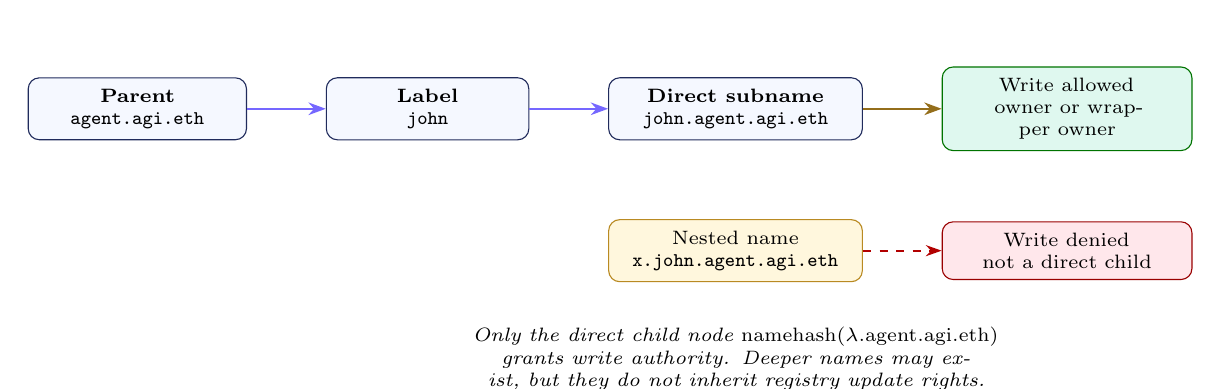
\begin{tikzpicture}[node distance=0.82cm and 1.0cm]
  \node[strongbox, text width=2.35cm] (parent) {Parent\\\code{agent.agi.eth}};
  \node[strongbox, right=of parent, text width=2.15cm] (label) {Label\\\code{john}};
  \node[strongbox, right=of label, text width=2.8cm] (child) {Direct subname\\\code{john.agent.agi.eth}};
  \node[goodbox, right=1.0cm of child, text width=2.75cm] (owner) {Write allowed\\owner or wrapper owner};
  \node[warnnode, below=1.0cm of child, text width=2.8cm] (nested) {Nested name\\\code{x.john.agent.agi.eth}};
  \node[badbox, right=1.0cm of nested, text width=2.75cm] (reject) {Write denied\\not a direct child};
  \draw[chainarrow] (parent) -- (label);
  \draw[chainarrow] (label) -- (child);
  \draw[gatearrow] (child) -- (owner);
  \draw[repairarrow] (nested) -- (reject);
  \node[font=\scriptsize\itshape, text width=9.2cm, align=center, below=0.45cm of nested] {Only the direct child node \(\mathrm{namehash}(\lambda.\mathrm{agent}.\mathrm{agi}.\mathrm{eth})\) grants write authority. Deeper names may exist, but they do not inherit registry update rights.};
\end{tikzpicture}}
\caption{Direct AGI Agent authorization. Only wallets controlling \(\lambda.\mathrm{agent}.\mathrm{agi}.\mathrm{eth}\) may update graph commitments for label \(\lambda\).}
\label{fig:ens}
\end{figure}

\section{On-Chain Object Model}
A skill capsule has a private and a public face. The private face contains method, reviewer notes, failure modes, model/tool traces, and sensitive operational context. The public face contains roots, hashes, pointers, proof levels, agent node, version, and events.

\begin{defbox}{Validated Skill Capsule}
A private capsule \(C\) contains the complete skill intelligence:
\[
\begin{aligned}
C=\langle &id,type,scope,method,evidenceSet,proofLevel,validators,\\
&replay,risk,limits,utility,rollback,version\rangle.
\end{aligned}
\]
Its public mainnet face \(\Pi(C)\) contains only commitments and verification handles:
\[
\begin{aligned}
\Pi(C)=\langle &agentNode,graphRoot,evidenceRoot,proofBundleRoot,\\
&schemaHash,proofLevel,version,uriSet,zkPolicyProof\rangle.
\end{aligned}
\]
\end{defbox}

The main commitment is:
\[
\begin{aligned}
\mathrm{skillCommitment}=H(&\mathrm{chainId},\mathrm{registry},\mathrm{agentNode},\mathrm{graphRoot},\\
&\mathrm{evidenceRoot},\mathrm{proofBundleRoot},\mathrm{schemaHash},\mathrm{version}).
\end{aligned}
\]
The graph root may be a Merkle root over canonicalized capsule fields; the evidence root may be a Merkle root over Evidence Docket claims, blocked claims, reviewer reports, and replay artifacts; the ProofBundle root may commit to returned work packages and validator verdicts.

\section{Zero-Knowledge Policy Proofs}
Zero-knowledge is useful when the system needs to prove that a hidden skill capsule satisfies a policy without revealing the underlying intelligence. V97.4 defines a \term{ZK Policy Proof} over a private witness:
\[
W=\langle C,E,P,V,K\rangle,
\]
where \(C\) is the skill capsule, \(E\) the Evidence Docket, \(P\) the ProofBundle set, \(V\) the validator attestations, and \(K\) the encryption/key policy. Public inputs include the roots and policy identifier:
\[
\begin{aligned}
X=\langle &graphRoot,evidenceRoot,proofBundleRoot,schemaHash,\\
&proofLevel,agentNode,policyHash\rangle.
\end{aligned}
\]
The proof statement is:
\[
\mathrm{Verify}_{zk}(X,\pi)=1 \Rightarrow
\begin{cases}
\text{capsule commits to } graphRoot,\\
\text{evidence commits to } evidenceRoot,\\
\text{ProofBundles commit to } proofBundleRoot,\\
\text{validator quorum is satisfied,}\\
\text{blocked claims are excluded,}\\
\text{proof level threshold is met,}\\
\text{rollback condition exists.}
\end{cases}
\]

\begin{figure}[t]
\centering
\resizebox{0.96\linewidth}{!}{%
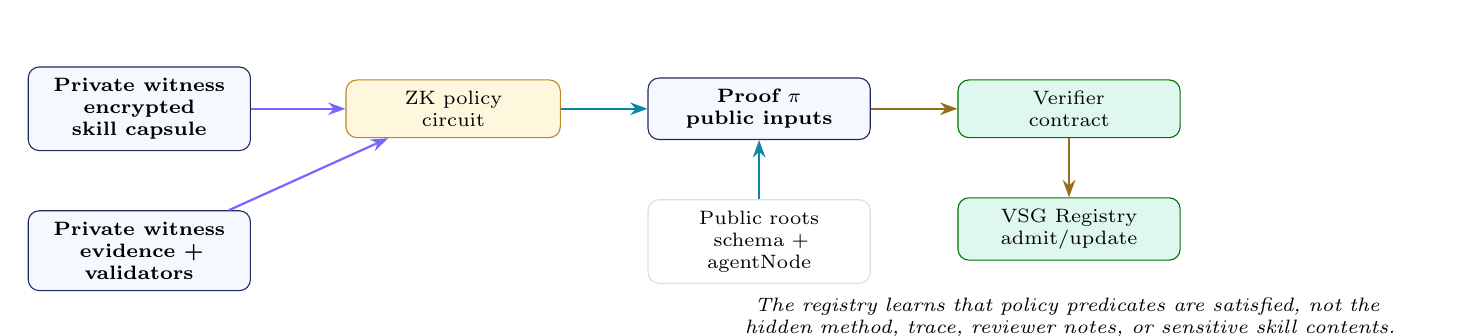
\begin{tikzpicture}[node distance=0.75cm and 0.75cm]
  \node[strongbox, text width=2.4cm] (capsule) {Private witness\\encrypted skill capsule};
  \node[strongbox, below=of capsule, text width=2.4cm] (evidence) {Private witness\\evidence + validators};
  \node[warnnode, right=1.2cm of capsule, text width=2.3cm] (circuit) {ZK policy\\circuit};
  \node[strongbox, right=1.1cm of circuit, text width=2.4cm] (proof) {Proof \(\pi\)\\public inputs};
  \node[goodbox, right=1.1cm of proof, text width=2.4cm] (verifier) {Verifier\\contract};
  \node[goodbox, below=of verifier, text width=2.4cm] (registry) {VSG Registry\\admit/update};
  \node[nodebox, below=of proof, text width=2.4cm] (publics) {Public roots\\schema + agentNode};
  \draw[chainarrow] (capsule) -- (circuit);
  \draw[chainarrow] (evidence) -- (circuit);
  \draw[proofarrow] (circuit) -- (proof);
  \draw[proofarrow] (publics) -- (proof);
  \draw[gatearrow] (proof) -- (verifier);
  \draw[gatearrow] (verifier) -- (registry);
  \node[font=\scriptsize\itshape, text width=9.0cm, align=center, below=0.35cm of registry] {The registry learns that policy predicates are satisfied, not the hidden method, trace, reviewer notes, or sensitive skill contents.};
\end{tikzpicture}}
\caption{Zero-knowledge policy proof. Hidden skill intelligence remains private; public contracts verify eligibility predicates over commitments.}
\label{fig:zk}
\end{figure}

\section{Validator Attestations}
Validators and AGI Agents should sign typed statements rather than ambiguous strings. V97.4 uses an EIP-712 style typed object:
\begin{lstlisting}
SkillAttestation {
  bytes32 agentNode;
  bytes32 skillCommitment;
  bytes32 graphRoot;
  bytes32 evidenceRoot;
  bytes32 proofBundleRoot;
  uint8   proofLevel;
  bytes32 policyHash;
  uint64  expiresAt;
  string  verdict;      // supported | blocked | needs-more-proof
}
\end{lstlisting}
The attestation root becomes part of the ZK witness or Evidence Docket root. This lets validators attest privately, publicly, or selectively depending on the proof level.

\section{Registry Surface}
The minimal registry exposes three authority-changing operations:
\begin{lstlisting}[language=C]
registerSkill(labelhash, graphRoot, graphURI,
              evidenceRoot, evidenceURI,
              proofBundleRoot, proofBundleURI,
              proofLevel, schemaHash, zkProof);

supersedeSkill(oldSkillId, newRoots, newURIs, proofLevel,
               schemaHash, zkProof);

revokeSkill(skillId, reasonURI);
\end{lstlisting}
The caller must own the direct AGI Agent subname for the label. The registry emits append-auditable events and never erases provenance. Supersession and revocation preserve history while removing or replacing future influence.

\begin{figure}[t]
\centering
\resizebox{0.95\linewidth}{!}{%
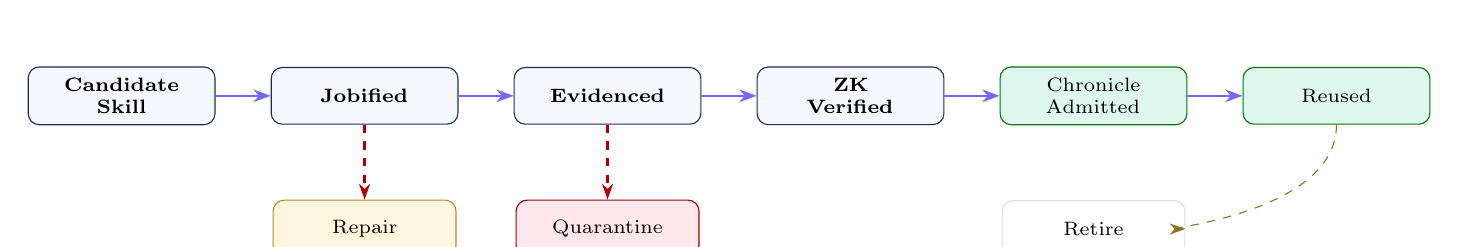
\begin{tikzpicture}[node distance=0.7cm and 0.7cm]
  \node[strongbox, text width=1.95cm] (candidate) {Candidate\\Skill};
  \node[strongbox, right=of candidate, text width=1.95cm] (jobified) {Jobified};
  \node[strongbox, right=of jobified, text width=1.95cm] (evidenced) {Evidenced};
  \node[strongbox, right=of evidenced, text width=1.95cm] (verified) {ZK\\Verified};
  \node[goodbox, right=of verified, text width=1.95cm] (admitted) {Chronicle\\Admitted};
  \node[goodbox, right=of admitted, text width=1.95cm] (reused) {Reused};
  \node[warnnode, below=0.95cm of jobified, text width=1.9cm] (repair) {Repair};
  \node[badbox, below=0.95cm of evidenced, text width=1.9cm] (quarantine) {Quarantine};
  \node[nodebox, below=0.95cm of admitted, text width=1.9cm] (retire) {Retire};
  \draw[chainarrow] (candidate) -- (jobified);
  \draw[chainarrow] (jobified) -- (evidenced);
  \draw[chainarrow] (evidenced) -- (verified);
  \draw[chainarrow] (verified) -- (admitted);
  \draw[chainarrow] (admitted) -- (reused);
  \draw[repairarrow] (jobified) -- (repair);
  \draw[repairarrow] (evidenced) -- (quarantine);
  \draw[softarrow] (reused) .. controls +(0,-1.5cm) and +(0.8cm,0) .. (retire);
\end{tikzpicture}}
\caption{Encrypted and zk-verified lifecycle. Mainnet authority appears only after authorization, evidence, zk policy verification, and Chronicle admission.}
\label{fig:lifecycle}
\end{figure}

\section{Security Invariants}
The system is designed around security invariants rather than interface promises.

\begin{table}[h]
\centering
\small
\begin{tabularx}{\linewidth}{p{0.27\linewidth}Y}
\toprule
\textbf{Invariant} & \textbf{Meaning} \\
\midrule
Direct-agent write authority & Only the owner of \(\lambda.\mathrm{agent}.\mathrm{agi}.\mathrm{eth}\) may mutate records for \(\lambda\). \\
No plaintext intelligence & Sensitive method, trace, reviewer notes, and domain evidence are never stored on-chain as plaintext. \\
Commitment consistency & On-chain roots must match canonicalized encrypted/off-chain payloads. \\
ZK-gated hidden claims & Hidden skill properties may grant authority only through verified policy proofs. \\
Chronicle non-contamination & Unproven or out-of-scope skills cannot influence future missions. \\
Supersession over deletion & Invalidated skills are superseded, revoked, or retired without erasing provenance. \\
\bottomrule
\end{tabularx}
\caption{Security invariants for the encrypted mainnet Validated Skill Graph.}
\label{tab:invariants}
\end{table}

\section{Threat Model}
\begin{table}[h]
\centering
\small
\begin{tabularx}{\linewidth}{p{0.22\linewidth}Y Y}
\toprule
\textbf{Threat} & \textbf{Failure mode} & \textbf{Control} \\
\midrule
Name spoofing & A wallet claims to be an AGI Agent without owning the direct subname. & ENS Registry and NameWrapper owner checks. \\
Nested-subname escalation & A deeper subname tries to inherit root authority. & Direct-subname node computation only. \\
Ciphertext leakage & Encrypted intelligence is copied forever from public chain data. & Minimize on-chain ciphertext; use strong encryption and key governance. \\
Weak proof circuit & ZK proof omits a required predicate. & Circuit audits, public policy hash, test vectors, formal acceptance tests. \\
Validator collusion & Attesters approve weak skills. & Quorum, reputation, challenge windows, delayed outcome checks. \\
Memory contamination & Unsupported skill enters future missions. & Chronicle gate and non-contamination invariant. \\
Key compromise & Decryption keys leak. & Rotation, threshold access, revocation, supersession, and encrypted capsule retirement. \\
\bottomrule
\end{tabularx}
\caption{Threats and controls. The central risk is not just data leakage; it is unauthorized authority over future work.}
\label{tab:threats}
\end{table}

\section{Implementation Checklist}
A mainnet launch should not be treated as a UI deployment. It is a cryptographic and institutional system deployment.
\begin{enumerate}
  \item Verify ownership and governance of \code{agent.agi.eth}.
  \item Deploy or audit the VSG Registry contract.
  \item Confirm ENS Registry and NameWrapper addresses for the target chain.
  \item Canonicalize the skill-capsule JSON schema.
  \item Choose storage mode: commitment-only, encrypted URI, encrypted on-chain capsule, or zk-verified hidden capsule.
  \item Build test vectors for labelhash, namehash, agentNode, roots, and schema hashes.
  \item Audit ZK circuits for proof-level, quorum, blocked-claim, replay, and rollback predicates.
  \item Define EIP-712 attestation domain, typed data, expiry, and revocation policy.
  \item Run adversarial tests: spoofed subname, nested subname, wrong owner, stale proof, bad capsule, invalid proof, revoked skill.
  \item Publish deployment address, ABI, schema hash, policy hash, and reviewer guide.
\end{enumerate}

\section{Evaluation Program}
V97.4 should be evaluated under three categories.

\textbf{Authorization tests.} A direct owner of \code{john.agent.agi.eth} can register; a non-owner cannot; a wrapper owner can register; a nested subname cannot inherit authority.

\textbf{Privacy tests.} Plaintext method and reviewer notes do not appear on-chain. Ciphertext capsules decrypt only for authorized recipients. ZK proofs verify policy predicates while hiding witness fields.

\textbf{Capability tests.} A skill commitment cannot influence future missions until Chronicle admission is present. Superseded or revoked skills are excluded from reuse. Proof levels change validator burden and accepted evidence thresholds.

\section{Claim Boundary}
This paper does not claim that encrypted on-chain storage is automatically safe. Public-chain ciphertext is permanent and subject to future cryptanalysis and key compromise. For high-sensitivity intelligence, the preferred pattern is encrypted off-chain storage plus on-chain commitments and zk policy proofs. The encrypted on-chain capsule mode is reserved for compact, carefully classified records whose long-term exposure risk has been accepted by governance.

The paper also does not claim achieved AGI, achieved ASI, empirical state of the art, legal certification, financial advice, guaranteed ROI, live settlement, wallet safety, or production authority.

\section{Conclusion}
GoalOS V97.4 turns the Validated Skill Graph into an authorized, privacy-preserving mainnet memory substrate. Direct AGI Agents write. Independent validators attest. Ethereum stores commitments, optional ciphertext capsules, schema hashes, policy proofs, and version events. Zero-knowledge proofs let the system verify that hidden skill intelligence satisfies policy without exposing the intelligence itself. Chronicle gates preserve the central law: future work may rely only on capability that was proven, authorized, privacy-preserved, and safe to reuse.

\begin{thesisbox}{Final line}
The graph should not remember what was merely said. It should remember only what was proven, authorized, privacy-preserved, and safe to reuse.
\end{thesisbox}

\begin{thebibliography}{9}
\bibitem{vsg} Montreal.AI Research. \emph{GoalOS: The Validated Skill Graph.} Research edition, 2026.
\bibitem{v85} Montreal.AI Research. \emph{GoalOS V85: A Unified Sovereign Proof Economy Operating System.} Research draft, 2026.
\bibitem{ensnames} ENS Documentation. \emph{Name Processing: namehash and labelhash.} \url{https://docs.ens.domains/resolution/names/}
\bibitem{ensdeploy} ENS Documentation. \emph{Deployments and mainnet registry.} \url{https://docs.ens.domains/learn/deployments/}
\bibitem{namewrapper} ENS Documentation. \emph{Name Wrapper overview.} \url{https://docs.ens.domains/wrapper/overview/}
\bibitem{eip712} Ethereum Improvement Proposal 712. \emph{Typed structured data hashing and signing.} \url{https://eips.ethereum.org/EIPS/eip-712}
\bibitem{groth16} Jens Groth. \emph{On the Size of Pairing-Based Non-interactive Arguments.} EUROCRYPT, 2016.
\bibitem{zcash} Eli Ben-Sasson et al. \emph{Zerocash: Decentralized Anonymous Payments from Bitcoin.} IEEE S\&P, 2014.
\end{thebibliography}

\end{document}
